\documentclass[10pt,a4paper,twocolumn]{article}
\usepackage[font=small,skip=0pt]{caption}

%\renewcommand{\section}{\section{\bold{#1}}

\newcommand{\blankpage}{
\newpage
\thispagestyle{empty}
\mbox{}
\newpage
}

\usepackage[colorlinks=false]{hyperref}
\hypersetup{%
  colorlinks = true,
  linkcolor  = black
}
\usepackage{geometry}
\usepackage{url}
\usepackage{booktabs}

% maths
\usepackage{bm}
\usepackage{xspace}

% algorithms
\usepackage{algorithm,algpseudocode}
\newcommand{\init}{\textbf{Init}\xspace}
\newcommand{\dokw}{\textbf{do}\xspace}
\newcommand{\upon}{\textbf{Upon}\xspace}
\newcommand{\interface}{\textbf{Interface}\xspace}
\newcommand{\crash}{\textbf{Crash}\xspace}
\newcommand{\eventname}{\textbf{EventName}\xspace}
\newcommand{\procname}{\textbf{ProcName}\xspace}
\newcommand{\timename}{\textbf{TimeName}\xspace}
\newcommand{\state}{\textbf{State}\xspace}
\newcommand{\trigger}{\textbf{Trigger}\xspace}
\newcommand{\requests}{\textbf{Requests}\xspace}
\newcommand{\indications}{\textbf{Indications}\xspace}
\newcommand{\proc}{\textbf{Procedure}\xspace}
\newcommand{\timer}{\textbf{Timer}\xspace}
\newcommand{\call}{\textbf{Call}\xspace}
\newcommand{\return}{\textbf{Return}\xspace}
\newcommand{\setup}{\textbf{Setup}\xspace}
\newcommand{\periodic}{\textbf{Periodic}\xspace}
\newcommand{\cancel}{\textbf{Cancel}\xspace}
\newcommand{\receive}[3]{\textbf{Receiver} (\textbf{#1}, \emph{sender}, #2, #3)}
\newcommand{\send}[3]{\textbf{Send} (\textbf{#1}, \emph{dest}, #2, #3)}
\algblockdefx{Interface}{EndInterface}[1]{\interface #1}{\textbf{end} \interface}
\algblockdefx{AlgState}{EndAlgState}[1]{\state #1}{\textbf{end} \state}
\algblockdefx{Requests}{EndRequests}{\requests\textbf{:}}{}
\algblockdefx{Indications}{EndIndications}{\indications\textbf{:}}{}
\algblockdefx{Upon}{EndUpon}[1]{\upon #1 \algorithmicdo}{\textbf{end} \upon}
\algblockdefx{Trigger}{EndTrigger}[1]{\trigger #1}{\textbf{end} \trigger}
\algrenewcommand\textproc{}
\algrenewcommand\algorithmicprocedure{\textbf{Procedure}}
\makeatletter
\newlength{\trianglerightwidth}
\settowidth{\trianglerightwidth}{$\triangleright$~}
\algnewcommand{\LineComment}[1]{\State \texttt{//} \textit{#1}}
\algnewcommand{\LineCommentCont}[1]{\State%
  \parbox[t]{\dimexpr\linewidth-\ALG@thistlm}{\hangindent=\trianglerightwidth \hangafter=1 \strut$\triangleright$ \emph{#1}\strut}}
\makeatother
\newcommand{\farg}[1]{\ensuremath{\textbf{arg}_{#1}}\xspace}

% % Fonts
\usepackage{times}
\usepackage[T1]{fontenc}

\def\course{Cloud Computing Systems}
\def\coursePT{Sistemas de Computação Cloud}

\def\titulo{TuKano Implementation leveraging Kubernetes}
\title{\titulo}

\def\data{\today}
\date{\data}



% Set your name here
\def\name{Filipe Colla David and Victor Ditadi}
\def\institution{
Departamento de Inform{\'a}tica\\
Faculdade de Ciências e Tecnologia\\
Universidade NOVA de Lisboa}

\author{\name\\ \institution}

% The following metadata will show up in the PDF properties
\hypersetup{
  colorlinks = true,
  urlcolor = black,
  pdfauthor = {\name},
  pdfkeywords = {Pseudocode, Link Abstractions}
  pdftitle = {\course: Lab 1 Problem},
  pdfsubject = {\course},
  pdfpagemode = UseNone
}

\geometry{
  body={6.5in, 9.0in},
  left=1.0in,
  top=1.0in
}

% Customize page headers
\pagestyle{myheadings}
\markright{\course - Project TuKano Kubernetes Report}
\thispagestyle{empty}

% Custom section fonts
\usepackage{sectsty}

\usepackage{amsmath}
\usepackage{listings}
\usepackage{graphicx}

\sectionfont{\rmfamily\mdseries\Large\textbf}
\subsectionfont{\rmfamily\mdseries\itshape\large}

\begin{document}

\pagenumbering{arabic} 

\maketitle

\section{Introduction}
\label{sec:intro}
This document explains the implementation of the TuKano App leveraging Kubernetes{\cite {kubernetes}}. TuKano is a social network inspired in existing video sharing services, such as TikTok or Youtube Shorts. TuKano users can upload short videos to be viewed (and liked) by other users of the platform. The social network aspect of TuKano resides on having users follow other users, as the main way for the platform to populate the feed of shorts each user can visualize.
\par The implementation of the application is divided will be divided into several microservices that will be managed by a Kubernetes Cluster. The performance analysis of using the different services will be presented in Section \ref{sec:Perf}.

\section{TuKano Application}
\label{sec:application}
This application can be divided basically into three major logical components, Users, Shorts and Blobs. 
\par The Users component holds all the logic for creating a user, deleting a user.
\par The Shorts component holds all the logic for creating, deleting a Short. A Short is a data model that holds the information for regarding a specific video, that was uploaded to the application. This component also contains the logic for following and liking other users/shorts.
\par The Blobs component holds all the logic for creating, deleting a blob.
\par These components are all related, however there's a stronger correlation between a Short and Blob, since every short contains the URL for a specific blob.

\section{Architecture and Behavior}
\label{sec:architecture}
This application is contained inside a Kubernetes Cluster, which manages the deployment, scaling, and operation of the microservices. As mentioned in the introduction, the application was divided into several microservices. 
\subsection{Components, Microservices}
As shown in Figure \ref{fig:tukano_architecture}, there are 5 major logical components, they are all defined as microservices, except for the ConfigMap, which complements the functionality of these microservices, additionally each one has a service to allow them to be reached via a DNS entry, managed by the Kubernetes Control Plane, instead of using the private cluster IpAddress of that instance.
\subsubsection{MINIO Service}
Minio\cite{minio} is a high-performance, distributed object storage system. It is designed to handle large amounts of unstructured data, such as photos, videos, log files, backups, and container images, which makes it a perfect replacement for Azure Blob Storage. It has a PVC (persistent volume claim) attached to avoid losing any data in the event of a restart of this deployment and contains a LoadBalancer that exposes this microservice to the outside of the cluster.

\subsubsection{PostgreSQL}
This microservice serves as the main database of the application, where user, shorts, following, and likes information is stored. It is defined as a StatefulSet, which is common practice in the industry. It also has a PVC attached to prevent data loss in the event of a StatefulSet restart.

\subsubsection{Redis Cache}
This microservice is used to cache frequently accessed information and cookies for user authentication.

\subsubsection{ConfigMap}
This is an individual resource that holds all the necessary environmental variables for the application.

\subsubsection{TuKano RestAPI}
This is a microservice containing the central REST API of this application. It holds the logic for creating and removing users, managing shorts, and storing blobs.
\par This microservice, in its essential form, consists of a pod with a Docker container that runs the Docker image defined in the repository of this project. This Docker image is built on top of \verb|tomcat:10.0-jdk17-openjdk-slim|, which allows it to run a Tomcat webserver that exposes a specific port for communication.
\par The communication with the database is handled using an Hibernate configuration and a JDBC Driver\cite{jdbc}. Communication with the MINIO storage is achieved through a MINIO Client\cite{minioClient}. Finally, uses Jedis\cite{jedis}, a Java client for Redis Cache, to interact with the caching service.



\begin{figure*}[h]
  \centering
  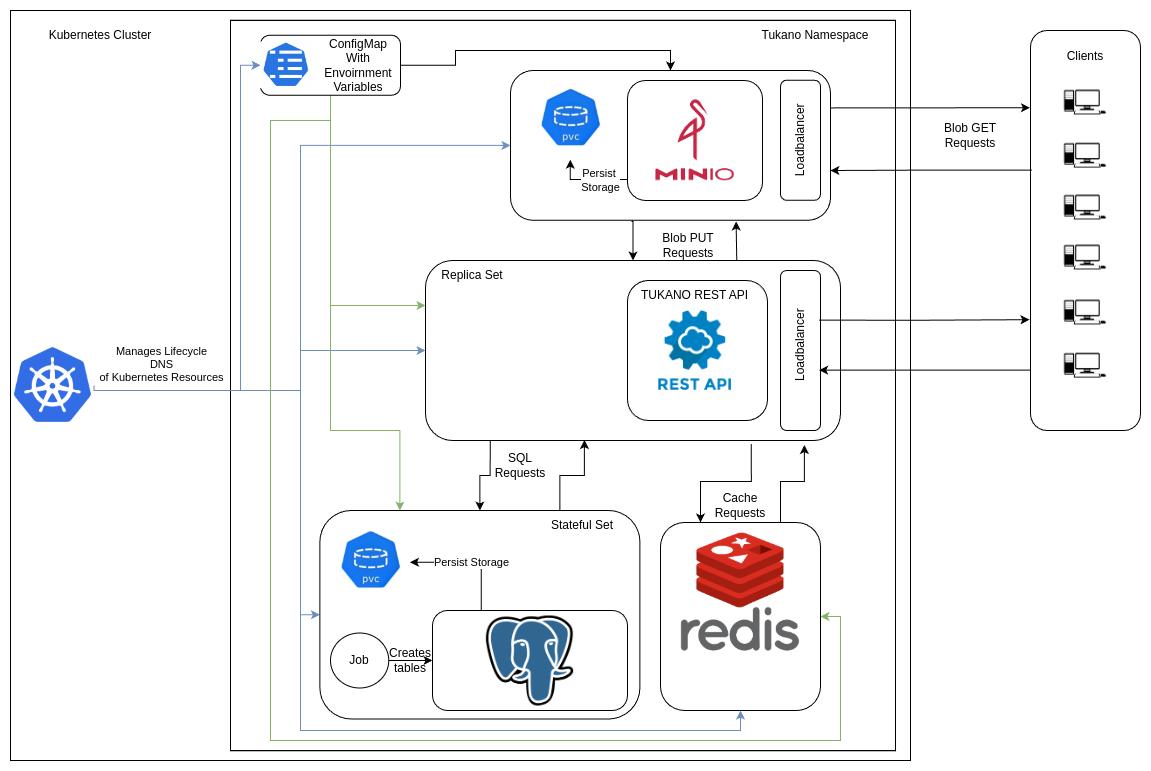
\includegraphics[width=\textwidth]{TuKanoArch.png}
  \caption{TuKano Application Architecture}
  \label{fig:tukano_architecture}
\end{figure*}


\subsection{Automated Deployment}
\label{sec:automatedDepl}
In order to easily deploy this application, a Makefile program was developed. A deployment of an application like this, requires several steps, and doing it manually is error prone.
The process:
\begin{enumerate}
  \itemsep0em 
  \item Compile the TuKano Application;
  \item Build the docker image and push it to the DockerHub;
  \item Update the docker image on the TuKano microservice yaml definition;
  \item Deploy every microservice available.
\end{enumerate}
As mentioned previously this process is mostly automated, however, there are some values from the ConfigMap that must be changed manually.

\subsection{Behavior}
\label{sec:behaviour}
Each microservice, upon starting will have access to the "Secrets" ConfigMap that holds all the necessary environmental variables for the configuration of their state. This includes the connections strings to the Database, Cache and Minio Storage, as well as some passwords and additional configuration parameters. However, as previously mentioned, there is a parameter on the ConfigMap that must be changed, the external URL of the MINIO LoadBalancer. Since the attribution of this URL is dynamic, this manual extra step is needed in order to ensure that the shorts will be stored with the right address to its blob. This is achieved by editing the "Secrets" ConfigMap, and deleting the TuKano RestAPI pod afterwards, so that it updates it's values from the new ConfigMap.
\par Once this initial configuration is complete, the application is ready to accept requests. As shown in Figure \ref{fig:tukano_architecture}, the TuKano Rest API is the central communication of the whole ecosystem, it communicates with the Database and the Cache to store the relational information of the users activity, and communicates with the MINIO storage microservice to store the blobs. The MINIO makes this blobs available through a LoadBalancer that exposes the service to the outside of the Kubernetes cluster.

\section{Performance Analysis}
\label{sec:Perf}
In this section there will be an analysis of the performance difference of the four different scenarios. To conduct these performance tests, the framework Artillery\cite{artillery} was used. This framework allows the programmer to test its application by creating several HTTP requests, once the experiment with the configured HTTP requests terminates, the framework outputs several statistics with the results obtained from the experiment.
\par In the particular case of this application, for each scenario three tests were conducted:
\begin{itemize}
  \item \textbf{Register Users}: Consists in inserting and requesting multiple users. This test was divided into register an user, get the user registered, and update that same user, repeated for 200 users, over the span of 100 seconds. 
  \item \textbf{Upload Shorts}: Consists in uploading and requesting multiple shorts. This test was divided into creating a short, and uploading a blob for that respective short. This process was repeated for 30 "shorts" over the span of 10 seconds, starting with one client\footnote{A client represents a simulated human that makes requests to complete the operations of the test}/second ramping up to five clients/second
  \item \textbf{Realistic Flow}: Consists in making several HTTP requests to the application to test all the endpoints. Ran multiple requests over the span of 10 seconds, starting with one client/second ramping up to five clients/second.
\end{itemize}
  
\subsection{Register User}
\label{sec:RegisterUser}
In the Figure \ref{fig:register_statistics}, we can observe the average response time and the minimum response time across the different scenarios. 
\par When using a cache (nosql\_cache and sql\_cache) label we can observe that the average response time is lower when compared to the scenarios that don't use a cache (nosql\_nocache and sql\_nocache). This is an excepted behavior, since the cache stores, ideally, frequently used information and provides a faster response time when compared to a request made directly to the database. This is due to the reason of caches running in memory, and have much faster access times to the required data. However, they can't hold as much data as a normal database, that utilizes a disk to store its data, and cache misses will occur when the cache is full, which will represent a penalty for accessing the required data.
\par There is also a significant difference between using SQL scenarios (sql\_nocache and sql\_cache) and NoSQL scenarios (nosql\_nocahce and nosql\_cache), this is usually the case since SQL queries are slower than NOSQL queries\cite{sqlNOSQLPerformance}.
% \begin{figure}[h]
%   \centering
%   \includegraphics[width=\linewidth]{register_statistic.png}
%   \caption{Register Response Time With Different Scenarios}
%   \label{fig:register_statistics}
% \end{figure}

\subsection{Upload Shorts}
\label{sec:UploadShorts}
In the Figure \ref{fig:endpoints_comparison} we can see that the average doesn't change significantly over the four scenarios, this is the case since they all use the same mechanism to store shorts and blobs, and the cache is not being used to store blobs.

% \begin{figure}[h]
%   \centering
%   \includegraphics[width=\linewidth]{response_times_comparison2.png}
%   \caption{Average Response time for uploading Shorts}
%   \label{fig:endpoints_comparison}
% \end{figure}

\subsection{Realistic Flow}
\label{sec:realisticFlow}
In this particular case there were some issues with testing, and some endpoints returned an HTTP response of 404 or 500, this issue wasn't discovered until the new extensive tests were done which was after the submission of the code. The functionalities affected were the ones related to likes, and getting shorts (note that this was correctly tested in the (\ref{sec:UploadShorts})). The true reason is yet unknown, however it might be due to some incompatibility between our implementation and the tests used, since the tests we ran previously detected no issue. Remains an objective for Future Work (\ref{sec:FutWork}).
\par Despite the encountered issues, there is still some valuable information to analyze in Figure \ref{fig:realistic_flow}\footnote{Note: Due to the issues encountered, download\_short and like\_short are not valid results}, overall we can observe that using cache guarantees a faster average response time (when its being utilized, it's not the case for uploading blobs).

% \begin{figure}[h]
%   \centering
%   \includegraphics[width=\linewidth]{realist_statistics_combined.png}
%   \caption{Average Response time for uploading Shorts}
%   \label{fig:realistic_flow}
% \end{figure}

\section{Future Work}
\label{sec:FutWork}
As for future work, the main thing needed would be to change the ConfigMap that holds all the information for the microservices, including the passwords to a Kubernetes Secret, which much more secure for sharing sensitive information.

\section{Challenges and Limitations}
\label{sec: challengesLimit}
\par Getting started with the development of the project presented itself as a great challenge for non Linux users. Multiple non compiler errors were found when testing using MacOS, which wrongly influenced some problem solving decisions, leading to considerable setbacks. A solution to those problems has yet to be found.
\par Inconsistencies with the Azure Could infrastructure also influenced the course of the development of this project.

\section {Conclusions}
\label{sec:Conc}
As mentioned in the Performance Analysis Section \ref{sec:Perf}, using a cache can be beneficial when developing an application like this, however, in the Azure Cloud System, this represents an added cost. Using SQL does improve the structuring of the databases, as mentioned in section \ref{sec:RegisterUser}, this can have a negative impact on latency\cite{sqlNOSQLPerformance}.

\bibliography{biblio}
\bibliographystyle{abbrv}

\end{document}